\documentclass[10pt,twocolumn,letterpaper]{article}

\usepackage{cvpr}
\usepackage{times}
\usepackage{epsfig}
\usepackage{graphicx}
\usepackage{amsmath}
\usepackage{amssymb}

% Include other packages here, before hyperref.

% If you comment hyperref and then uncomment it, you should delete
% egpaper.aux before re-running latex.  (Or just hit 'q' on the first latex
% run, let it finish, and you should be clear).
\usepackage[breaklinks=true,bookmarks=false]{hyperref}

\cvprfinalcopy % *** Uncomment this line for the final submission

\def\cvprPaperID{****} % *** Enter the CVPR Paper ID here
\def\httilde{\mbox{\tt\raisebox{-.5ex}{\symbol{126}}}}

% Pages are numbered in submission mode, and unnumbered in camera-ready
%\ifcvprfinal\pagestyle{empty}\fi
\setcounter{page}{1}
\begin{document}

%%%%%%%%% TITLE
\title{Object recognition \& Computer vision \\ Final report - MVA 2015 \\ \textit{Functional Maps: A Flexible Representation of Maps Between Shapes}}

\author{PAUMIER Nicolas\\
ENS Cachan\\
{\tt\small paumiern.ensimag@gmail.com }
% For a paper whose authors are all at the same institution,
% omit the following lines up until the closing ``}''.
% Additional authors and addresses can be added with ``\and'',
% just like the second author.
% To save space, use either the email address or home page, not both
\and
THIS Alexandre\\
ENS Cachan\\
{\tt\small alexandre.this@gmail.com}
}

\maketitle
%\thispagestyle{empty}

%%%%%%%%% ABSTRACT
\begin{abstract} %NICO
\cite{ovs} presented a novel approach for non-rigid shape matching. Their approach relies on the concept of functional representation of the mapping between shapes. In this paper, the author say that their method provides a compact, stable, multi-scale aware representation yielding state of the art result. We re-implemented their method and tried to do an analysis of the different parameters as well as the post-processing steps described. This representation is indeed compact but relies strongly on the descriptor function used. However the use of traditional 3D shape descriptor as WKS and HKS combined yield impressive results. Moreover the refinement step described in the original paper seems to be a very important step of the method as it strongly improves the initial map.
\end{abstract}

%%%%%%%%% BODY TEXT

\section{Introduction} %ALEX
%Statement of the problem, quick recap of previous work
One area of interest of shape analysis is the problem of shape matching. The general statement of this problem would be the following : \textit{Given two shapes $S_{1}$ and $S_{2}$, find a mapping that bind the elements of the two shapes}. Once the mapping has been found, there is a wide range of applications that can use it. For example, segmentation transfer can be used in order to find the segmentation of a deformed shape given a segmentation of the initial shape and a mapping between the initial and the deformed shape. Other applications exists such as motion transfer, shape interpolation or statistical modeling for example.

The goal of the studied paper is to address the general problem of non rigid shape matching. This problem is quite difficult for several reasons. In contrary to rigid shape matching, the parameters of the transformation are not only tied to rotation and translation anymore. The space of parameters is much higher and it is expensive to optimize the transformation based only on point correspondences. 

Several papers try to avoid doing this by using different methods that are trying to use only some landmark correspondences in order to optimize the transformation, and establish a dense correspondence afterwards. The studied paper is instead focusing on the representation for the correspondences. The goal was to define a compact representation of shape mapping that allows efficient manipulation, that is multiscale and that can lead to simple optimization problems.


\section{Method} %NICO
%Description de la fonctional map
Instead of putting in correspondence points on the shapes, \cite{ovs} propose to consider mapping between functions defined on the shapes. 
Let $T : M \rightarrow N$ be a bijective mapping between manifolds $M$ and $N$. Given a scalar function $f: M \rightarrow \mathbb{R}$, we obtain the corresponding function $g : N \rightarrow \mathbb{R}$ by composition, $g=f \circ T^{-1}$. This induced transformation, $T_F : \mathcal{F}(M,\mathbb{R})\rightarrow \mathcal{F}(N,\mathbb{R})$ where $\mathcal{F}(\dot,\mathbb{R})$ denote a generic space of real-valued function, is called the functional representation of the mapping $T$. 
If $\mathcal{F}(M,\mathbb{R})$ and $\mathcal{F}(N,\mathbb{R})$ has a Basis \{$\phi_i^M$\} and \{$\phi_j^N$\}, then any function $f$ on $M$ and $g$ on $N$ can be represented as a vector $a=(a_i)_{i \in \mathbb{N}}$ and $b=(b_j)_{i \in \mathbb{N}}$, s.t.
\begin{equation}
	f = \sum_{i=1}^{\infty}a_i \phi_i^M  \quad \quad g = \sum_{j=1}^{\infty}b_j \phi_j^N
\end{equation}
It follows the map $T_F$ can be represented as a (possibly infinite) matrix $C$ where $C_{i,j}=<T_F(\phi_i^M),\phi_j^N>$ and we can write $Ca=b$ from $T_F(f) = g$.

Then the goal is to first recover $C$ and then calculate $T$.

\paragraph{Choice of basis}

Ovsjanikov et al. use the first $n$ Laplace-Beltrami eigenfunctions as the basis for their functional representation (\{$\phi_i^M$\} and \{$\phi_j^N$\}). This basis is compact and stable which allow us to consider a finite submatrix $C_{0..n \times 0..n}$ given a more compact representation of the map $T_F$. Moreover, the Laplace-Beltrami eigenfunctions are scale aware therefore satisfying the need of a multi-scale representation.

\paragraph{Recover matrix C} 
Many natural constraints on the map $T$ become linear constraints in its functional representation. The goal is to find enough constraints such that we can optimize $\underset{C}{\min}||Ca-b||$ where $a$ and $b$ are representation of corresponding functions $f$ and $g$. The differents constraints proposed by the authors are : 
\begin{description}
\item[Descriptor preservation] If $f$ and $g$ are point descriptors then they are approximately preserved by the mapping. We can phrase one linear constraint $Ca=b$ for each dimension of the descriptor.
\item[Landmark point and Segment correspondences] If we are given landmark point correspondences or correspondences between parts of shapes, we simply consider functions $f$ and $g$ that are describing those landmark points or parts of shapes and then phrase linear constraint $Ca=b$ for each correspondences.
\item[Regularization constraints] In order for $C$ to be associated with a point-to-point map between isometric shapes, $C$ must be a nearly-orthonormal map matrices. This property of $C$ is ensured by the commutativity of $C$ with the Laplace-Beltrami operator which can be written as a linear constraint $||R_FC-CS_F||=0$ where $R_F$ and $S_F$ are Laplace-Beltrami operators on $M$ and $N$.
\end{description}

After finding the matrix $C$ that best satifies the constraints, a point-to-point conversion is made to recover the map $T$.

\section{Implementation}
%TODO Recall what has been given, and what has been developped (given : LAB, fast_marching, recomputation of C, knn, ICP)
%Description de comment compute les constraints
\subsubsection*{Segmention} %NICO
In order to add segment correspondences constraints to the linear system, we implemented the persistence-based segmentation technique of \cite{Skraba} to obtain parts of both shapes and then manually find pair of parts between the 2 shapes.
%TODO add ref for Skraba et al
\subsubsection*{Constraints} %ALEX
In order to solve the linear system, one has to compute all the previously stated constraints (function preservation constraints, landmark preservation constraints, segment preservation constraints, and operator commutativity constraints). 

First, one has to notice that landmark and segment preservation constraints are special cases of function preservation constraints. Indeed, if one wants to add a landmark or a segment preservation constraints, one only need to define functions that are defined on the shapes that are corresponding to point or segment descriptor. In our implementation we used indicator function, distance function to landmarks, and a combination of indicator function and descriptor functions (a function that is $0$ everywhere, and that has the value of the descriptor on the segment for example). 

We know that the map $C$ bind the functions on the two spaces with the equation $Ca = b$. In order to get a regular linear equation, we rewrote it to have a regular linear equation $Ax = b$ where $x$ is the matrix $C$ written as a vector.

The second type of constraints that have been added to the system are the Operator Commutativity constraints. The Laplace-Beltrami operator is being preserved under isometries, therefore we have defined constraints for this operator. Moreover, we rewrote the equation $||L_{2}C - CL_{1}|| = 0$ ($L_{i}$ being the discrete Laplace-Beltrami operator defined on the shape $i$) into a regular linear system $Ax = b$ where $x$ is the matrix $C$ written as a vector. 

\subsubsection*{Weighting of the constraints}
As we have an overly determined system $Ax = b$. Instead of minimizing $e = Ax-b$, we want to minimize $e = W(Ax-b)$ where $W$ is a weight matrix. We can solve the problem by minimizing :
\begin{equation}
e^{T}e = (Ax-b)^{T}W^{T}W(Ax-b)
\end{equation}
This gives a system of linear equations in $x$ :
\begin{equation}
A^{T}W^{T}WAx = A^{T}W^{T}Wb
\end{equation}

\subsubsection*{Solving the system and post-processing}
Finally a linear least square solver has been used to obtain the map C. \\

We finally gravitated toward using the implementation of Pokrass et al. that provide a direct solution to the minimization problem \textit{minimize $||AX - B||$ s.t. $X'*X = Id$}. Note that the $X'*X = Id$ is the regularization constraints mentioned in our article. Our inspiration for the refinement of the map C (described in \cite{ovs} as similar to the ICP algorithm) is coming from the same open source code. Moreover, in order to find the point-to-point correspondences, we have used an open source kd-tree implementation.
%TODO add reference to licence of flann
%TODO add reference to pokrass, cf licence file



\section{Results} %ALEX
We first decided to test extensively how different constraints could affect the results obtained by this new representation. In order to do this, we used the constraints weighting to selectively choose which functions we wanted to use. Two type of descriptor functions were provided : the heat kernel signature, and the wave kernel signature. We also added segment constraints.

\begin{figure}[h]
\centering
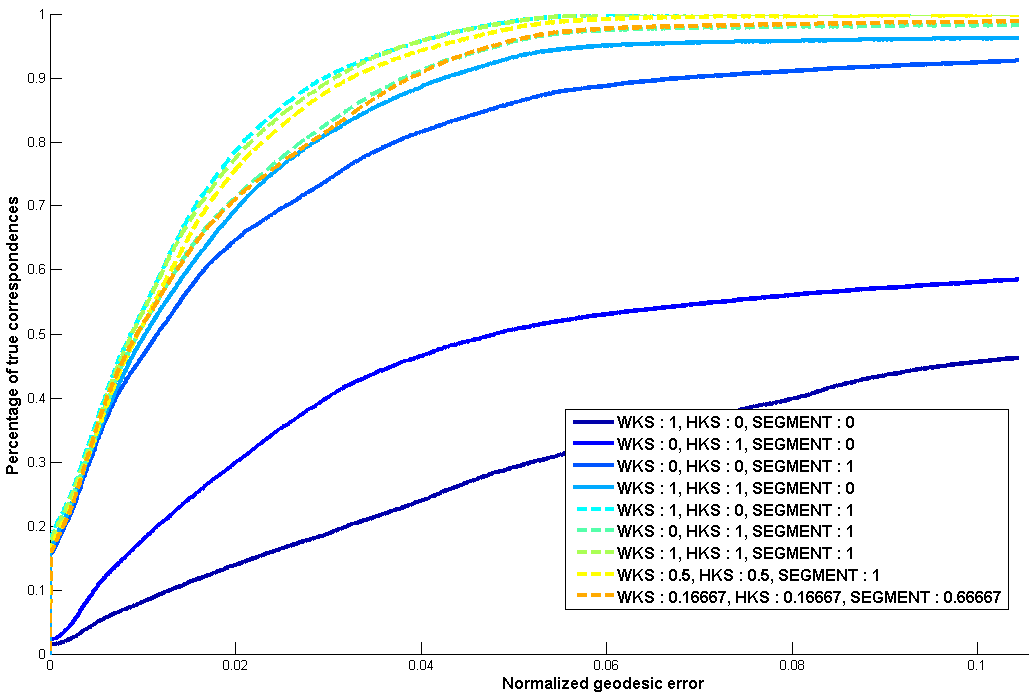
\includegraphics[width=.4\textwidth]{Images/weights.png}
\caption{Impact of the the different constraints on the error versus true correspondence}
\label{fig_weights}
\end{figure}

We can see on figure \ref{fig_weights} that using only one type of descriptor preservation constraints yield poor results. The best results asymptotically have been obtained using the three type of descriptor constraints equally weighted.

Moreover we wanted to see how the refinement affected the geodesic error. We can see on figure \ref{fig_refinement} that it has a huge impact on the results. One should consider using it extensively.

\begin{figure}[h]
\centering
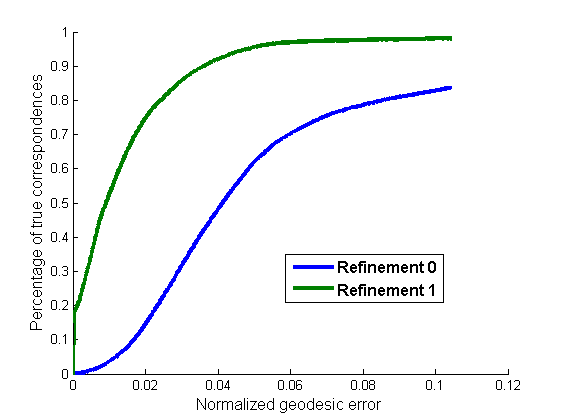
\includegraphics[width=.4\textwidth]{Images/refinement.png}
\caption{Impact of the refinement step on the error versus true correspondence}
\label{refinement}
\end{figure}

Finally we tested the impact of removing the Operator Commutativity constraints on the results as well as using the anisotropic Laplace-Beltrami operator. As the impact on the results are not obvious, we decided not to include them in this report as we couldn't find a proper explanation of the different results obtained.
 

\section{Discussions} %NICO/ALEX
We studied the method described in \cite{ovs}. that proposes a new representation for the non-rigid mapping of 3D shapes. This mapping relies on the concept of functional mapping that maps functions defined on a first shape onto an other shape. As we implemented this method, we have been able to confirm the fact that this new representation provides a compact representation of the complex transformation. We used only 40 eigenvalues (hence a map C of size $40x40$, and this was sufficient enough to get very good results). One of the main requirement of this method is to have good descriptor functions in order to compute the map, but we have shown that using the well known WKS and HKS actually yields very good results (those descriptor are also used to compute the segmentation). We tested the results on different transformation and even with strong isometry deformation we still obtain good results.

\begin{figure}[h]
\centering
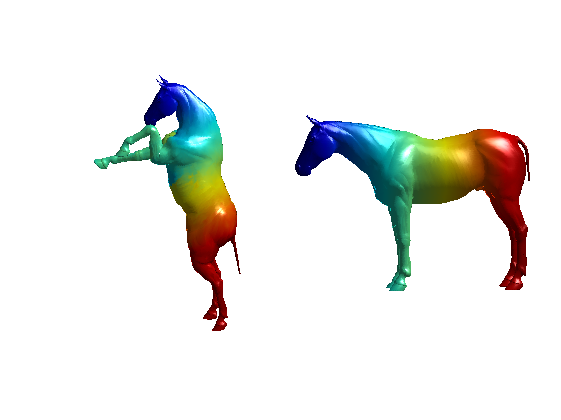
\includegraphics[width=.4\textwidth]{Images/full-constraints-iso1-3segments-horse.png}
\caption{Function transfer}
\label{refinement}
\end{figure}

\begin{figure}[h]
\centering
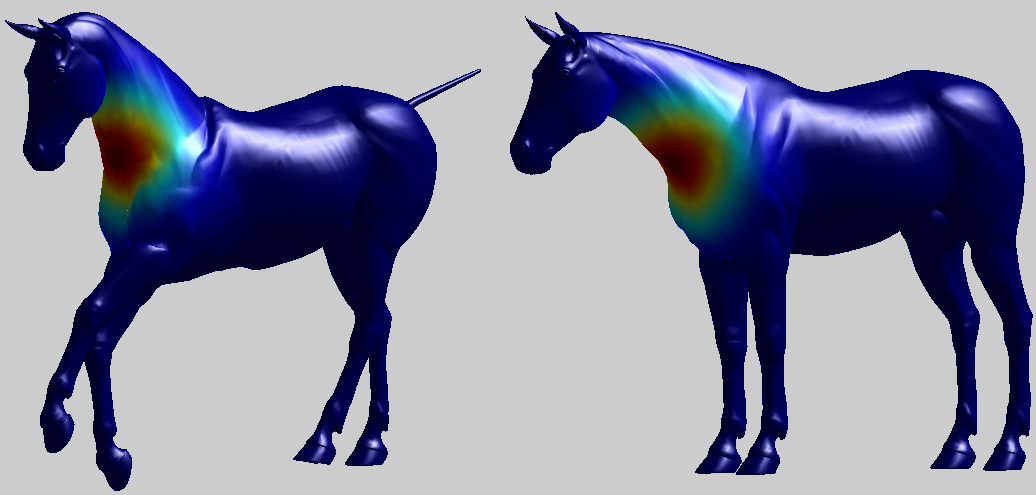
\includegraphics[width=.4\textwidth]{Images/pointTransfer.png}
\caption{Point transfer}
\label{refinement}
\end{figure}




\section*{Sources and Copyrights}
\begin{itemize}
\setlength\itemsep{0.01em}
\item{Our implementation : \url{https://github.com/Al-th/MVA_ObjectRecognitionProject}}
\item{LB Operator, WKS, HKS : Mathieu Aubry}
\item{Geodesic distance calculation : Gabriel Peyré}
\item{Kd-tree : Marius Muja and David G. Lowe}
\item{Inspiration for ICP : \url{https://github.com/jonathanpokrass/ShapeLAB}}
\end{itemize}

%-------

{\small
\bibliographystyle{ieee}
\bibliography{egbib}
}

\end{document}
